\section{Hướng dẫn điều khiển và Giao diện người dùng}

\subsection{Bảng phím điều khiển (Key Bindings)}
% [Gợi ý nội dung: Liệt kê các phím thao tác trong game]
\begin{table}[H]
    \centering
    \caption{Bảng phím điều khiển trong trò chơi}
    \label{tab:dieu_khien}
    \renewcommand{\arraystretch}{1.5}
    \begin{tabular}{|c|c|p{7cm}|}
        \hline
        \textbf{STT} & \textbf{Phím bấm} & \textbf{Chức năng / Hành động} \\
        \hline
        1 & \texttt{A} / Phím Mũi tên Trái & Di chuyển khối sang trái \\
        \hline
        2 & \texttt{D} / Phím Mũi tên Phải & Di chuyển khối sang phải \\
        \hline
        3 & \texttt{X} / \texttt{S} / Mũi tên Xuống & Tăng tốc độ rơi (Soft Drop) \\
        \hline
        4 & \texttt{W} / Phím Mũi tên Lên / Phím Cách & Xoay khối gạch (Rotate) \\
        \hline
        5 & \texttt{P} & Tạm dừng / Tiếp tục trò chơi (Pause/Resume) \\
        \hline
        6 & \texttt{Q} & Thoát khỏi trò chơi (Quit) \\
        \hline
    \end{tabular}
\end{table}

\subsection{Giao diện và Trải nghiệm người dùng}

\begin{figure}[H]
    \centering
    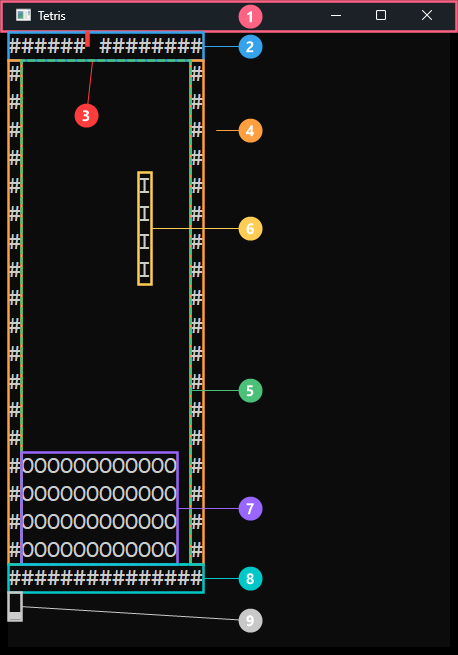
\includegraphics[height=11cm]{assest/tetris_00_chu_thich_giao_dien.png}
    \caption{Các khu vực trên giao diện trò chơi Tetris (ảnh chụp khi đang chơi)}
    \label{fig:ui_chu_thich}
\end{figure}

Bảng~\ref{tab:ui_khu_vuc} mô tả chi tiết từng khu vực được đánh số trong Hình~\ref{fig:ui_chu_thich}.

\begin{longtable}{|c|p{3.6cm}|p{11.2cm}|}
    \caption{Mô tả các khu vực trên giao diện}
    \label{tab:ui_khu_vuc} \\
    \hline
    \textbf{Số} & \textbf{Khu vực} & \textbf{Mô tả} \\
    \hline
    \endfirsthead
    \hline
    \textbf{Số} & \textbf{Khu vực} & \textbf{Mô tả} \\
    \hline
    \endhead
    1 & Thanh tiêu đề cửa sổ & Cửa sổ console chứa trò chơi. Chương trình không tự đặt tiêu đề, kích thước hay phông chữ; các thông số này phụ thuộc vào cấu hình console của máy đang chạy. \\
    \hline
    2 & Viền trên (hàng 0) & Dãy ký tự \texttt{\#} được tạo trong hàm \texttt{initBoard()}. Hàng này chỉ dùng để trang trí: hàm \texttt{canMove()} không kiểm tra va chạm với cạnh trên. \\
    \hline
    3 & Lỗ hổng trên viền trên & Là một lỗi hiển thị. Khối I xuất hiện tại $y = 0$ nên ghi đè lên ô \texttt{\#} ở cột 6. Khi khối di chuyển, hàm \texttt{boardDelBlock()} xóa ô đó thành khoảng trắng, nên viền trên bị thủng vĩnh viễn. \\
    \hline
    4 & Tường trái và tường phải & Cột 0 và cột 14 (ký tự \texttt{\#}). Hàm \texttt{canMove()} chặn không cho khối gạch đi ra ngoài hai cột này. \\
    \hline
    5 & Vùng chơi & Phần bên trong khung viền, gồm 13 cột $\times$ 18 hàng. Đây là nơi khối gạch rơi và được xếp chồng. Ô trống được hiển thị bằng khoảng trắng. \\
    \hline
    6 & Khối gạch đang rơi & Được vẽ bằng chữ cái tương ứng với loại khối (\texttt{I} hoặc \texttt{O}). Khối mới luôn xuất hiện ở vị trí $x = 5$, $y = 0$, tức là gần giữa phía trên vùng chơi. Mỗi chu kỳ 500\,ms khối rơi xuống 1 hàng. \\
    \hline
    7 & Các khối đã cố định & Khi không thể rơi tiếp, khối được ghi vĩnh viễn vào ma trận bằng hàm \texttt{block2Board()}. Khối đã cố định và khối đang rơi dùng cùng một ký tự, không có màu sắc hay dấu hiệu nào để phân biệt. \\
    \hline
    8 & Viền đáy (hàng 19) & Đáy của vùng chơi. Khối gạch dừng lại khi chạm hàng này hoặc chạm một khối đã cố định. \\
    \hline
    9 & Con trỏ console & Con trỏ nhấp nháy nằm ngay dưới bàn cờ vì chương trình không ẩn con trỏ. Con trỏ này không có chức năng trong trò chơi. \\
    \hline
\end{longtable}

Trong phiên bản hiện tại, giao diện \textbf{chưa có} các thành phần thường gặp của Tetris như bảng điểm, cấp độ, ô xem trước khối tiếp theo (\textit{Next Piece}) hay dòng hướng dẫn phím. Người chơi chỉ nhìn thấy bàn cờ.

\subsubsection{Giai đoạn 1: Bàn cờ lúc bắt đầu}

\begin{figure}[H]
    \centering
    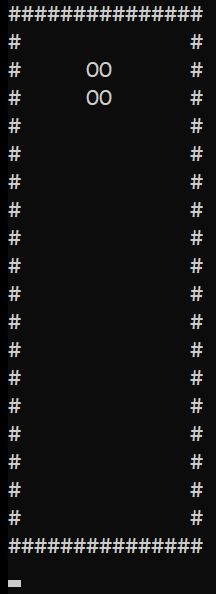
\includegraphics[height=9cm]{assest/tetris_01_bat_dau.png}
    \caption{Bàn cờ ngay sau khi khởi động trò chơi}
    \label{fig:ui_bat_dau}
\end{figure}

Khi chạy chương trình, trò chơi bắt đầu ngay lập tức mà không có màn hình chào hay menu. Hàm \texttt{initBoard()} tạo khung viền \texttt{\#} và một vùng chơi trống. Khối gạch đầu tiên (trong Hình~\ref{fig:ui_bat_dau} là khối \texttt{O}) xuất hiện ở giữa phía trên và bắt đầu rơi. Vì không có thông báo hay hướng dẫn nào, người chơi mới cần biết trước các phím \texttt{a}, \texttt{d}, \texttt{x}, \texttt{q} để điều khiển.

\subsubsection{Giai đoạn 2: Xếp gạch}

\begin{figure}[H]
    \centering
    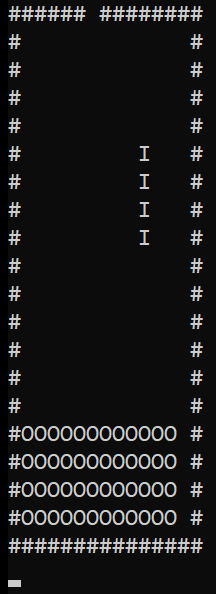
\includegraphics[height=9cm]{assest/tetris_02_xep_gach.png}
    \caption{Khối I đang được di chuyển sang phải để lấp khoảng trống}
    \label{fig:ui_xep_gach}
\end{figure}

Trong Hình~\ref{fig:ui_xep_gach}, người chơi đã xếp các khối \texttt{O} thành 4 hàng ở đáy, chỉ còn trống cột ngoài cùng bên phải. Khối \texttt{I} đang được di chuyển sang phải bằng phím \texttt{d} để lấp vào cột này. Mỗi lần bấm phím, khối dịch 1 ô; bấm \texttt{x} thì khối rơi thêm 1 hàng. Ở góc trên có thể thấy lỗ hổng trên viền (khu vực số 3) do một khối \texttt{I} xuất hiện trước đó để lại.

Khi xếp gạch, có hai điểm ảnh hưởng đến trải nghiệm:
\begin{itemize}
    \item \textbf{Chỉ có hai loại khối}: Lệnh \texttt{b = rand() \% 7} chỉ chọn trong 7 phần tử đầu của mảng \texttt{blocks}, gồm 2 khối \texttt{I} dựng đứng và 5 khối \texttt{O}. Vì vậy người chơi chỉ nhận được khối \texttt{O} (xác suất $5/7$) và khối \texttt{I} đứng (xác suất $2/7$). Các khối T, S, Z, J, L đã khai báo nhưng không bao giờ xuất hiện, và trò chơi cũng không có chức năng xoay khối.
    \item \textbf{Mỗi chu kỳ chỉ xử lý một phím}: Mỗi vòng lặp chỉ gọi \texttt{getch()} một lần, sau đó chờ 500\,ms. Nếu người chơi bấm nhiều phím liên tiếp, các phím này được đưa vào hàng đợi và xử lý dần, nên khối gạch phản hồi chậm hơn thao tác thực tế.
\end{itemize}

\subsubsection{Giai đoạn 3: Xóa dòng}

\begin{figure}[H]
    \centering
    \begin{minipage}{0.23\textwidth}
        \centering
        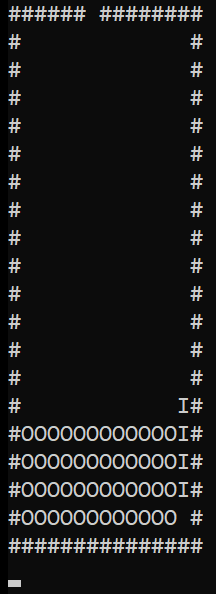
\includegraphics[width=\linewidth]{assest/tetris_03a_truoc_xoa_dong.png}\\
        \small (a) Trước khi xóa
    \end{minipage}\hfill
    \begin{minipage}{0.23\textwidth}
        \centering
        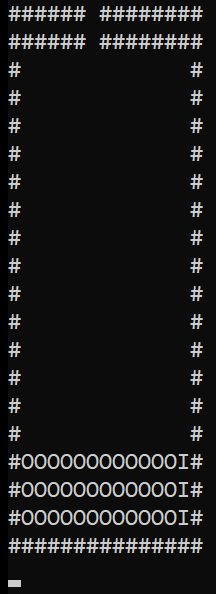
\includegraphics[width=\linewidth]{assest/tetris_03b_dang_xoa_dong.png}\\
        \small (b) Xóa hàng thứ 1
    \end{minipage}\hfill
    \begin{minipage}{0.23\textwidth}
        \centering
        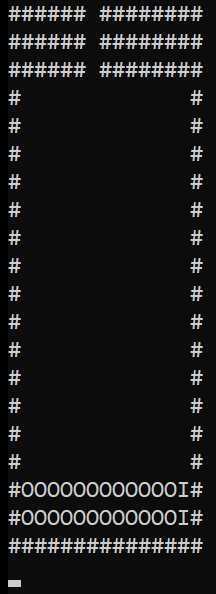
\includegraphics[width=\linewidth]{assest/tetris_03c_dang_xoa_dong.png}\\
        \small (c) Xóa hàng thứ 2
    \end{minipage}\hfill
    \begin{minipage}{0.23\textwidth}
        \centering
        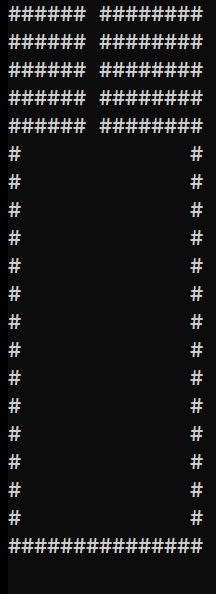
\includegraphics[width=\linewidth]{assest/tetris_03d_sau_xoa_dong.png}\\
        \small (d) Sau khi xóa 4 hàng
    \end{minipage}
    \caption{Quá trình xóa 4 hàng cùng lúc (Tetris)}
    \label{fig:ui_xoa_dong}
\end{figure}

Hình~\ref{fig:ui_xoa_dong} ghi lại lần xóa 4 hàng cùng lúc:
\begin{enumerate}[label=(\alph*)]
    \item Khối \texttt{I} sắp chạm đáy. Khi nó được cố định, cả 4 hàng dưới cùng sẽ đầy.
    \item Hàm \texttt{removeLine()} quét từ dưới lên. Mỗi khi gặp một hàng đầy, hàm dồn các hàng phía trên xuống 1 hàng, vẽ lại màn hình và dừng 200\,ms.
    \item Quá trình lặp lại với từng hàng đầy tiếp theo, nên các hàng biến mất lần lượt, tạo thành một hiệu ứng động đơn giản.
    \item Sau khi xóa xong, vùng chơi trống trở lại.
\end{enumerate}

Hiệu ứng từng bước giúp người chơi thấy rõ hàng nào vừa bị xóa. Tuy nhiên, giao diện không hiện điểm thưởng hay thông báo kiểu \textit{Single/Double/Triple/Tetris}, nên người chơi không nhận được phần thưởng nào cho việc xóa nhiều hàng cùng lúc.

Các ảnh chụp cũng cho thấy \textbf{một lỗi hiển thị} trong hàm \texttt{removeLine()}. Vòng lặp dồn hàng chạy đến \texttt{ii = 1} và gán \texttt{board[1] = board[0]}, tức là chép hàng viền \texttt{\#} xuống hàng 1. Vì vậy mỗi hàng bị xóa lại sinh thêm một hàng viền ở phía trên. Ở Hình~\ref{fig:ui_xoa_dong}(d), sau khi xóa 4 hàng, phía trên có tổng cộng 5 hàng \texttt{\#} và vùng chơi chỉ còn 14 hàng thay vì 18.

\subsubsection{Giai đoạn 4: Kết thúc trò chơi (Game Over)}

\begin{figure}[H]
    \centering
    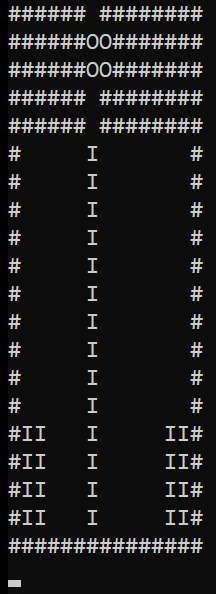
\includegraphics[height=9cm]{assest/tetris_04_ket_thuc.png}
    \caption{Trạng thái cuối khi khối gạch chạm nóc: trò chơi không hiện thông báo Game Over}
    \label{fig:ui_ket_thuc}
\end{figure}

Mã nguồn hiện tại \textbf{chưa có màn hình hay thông báo Game Over}. Hình~\ref{fig:ui_ket_thuc} là trạng thái cuối cùng khi các khối đã chồng lên đến vị trí xuất hiện khối mới:
\begin{itemize}
    \item Khối mới xuất hiện tại $y = 0$ mà không kiểm tra xem vị trí đó còn trống không. Nếu không rơi được, khối bị cố định ngay tại chỗ, đè lên các hàng \texttt{\#} ở phía trên (hai ô \texttt{OO} trong hình).
    \item Sau khi bị đè, hàng đó không còn khoảng trắng nên hàm \texttt{removeLine()} coi nó là hàng đầy và dồn hàng. Việc này lặp lại liên tục: màn hình vẫn nhấp nháy và vẽ lại nhưng người chơi không thể làm gì thêm. Trong lần chạy thử, trạng thái này kéo dài hơn 10 phút mà trò chơi không tự dừng.
    \item Cách duy nhất để thoát là bấm phím \texttt{q}. Chương trình không báo kết quả hay điểm số trước khi thoát.
\end{itemize}

\subsubsection{Đánh giá trải nghiệm người dùng}

\begin{table}[H]
    \centering
    \caption{Ưu điểm và hạn chế của giao diện hiện tại}
    \label{tab:ui_danh_gia}
    \renewcommand{\arraystretch}{1.4}
    \begin{tabular}{|p{7.6cm}|p{8.6cm}|}
        \hline
        \textbf{Ưu điểm} & \textbf{Hạn chế} \\
        \hline
        \begin{minipage}[t]{\linewidth}
        \begin{itemize}[leftmargin=*, nosep, before=\vspace{-0.7\baselineskip}]
            \item Giao diện đơn giản, nhẹ, chạy được trên mọi console Windows mà không cần thư viện đồ họa.
            \item Khung viền rõ ràng, người chơi dễ nhận ra ranh giới vùng chơi.
            \item Chỉ có 4 phím, dễ học.
            \item Hiệu ứng xóa từng hàng (200\,ms) giúp người chơi thấy kết quả thao tác.
        \end{itemize}
        \end{minipage}
        &
        \begin{minipage}[t]{\linewidth}
        \begin{itemize}[leftmargin=*, nosep, before=\vspace{-0.7\baselineskip}]
            \item Màn hình nhấp nháy vì \texttt{system("cls")} xóa và vẽ lại toàn bộ ở mỗi chu kỳ.
            \item Không có màu; khối đang rơi và khối đã cố định trông giống nhau.
            \item Không có điểm, cấp độ, khối tiếp theo, hướng dẫn phím hay thông báo Game Over.
            \item Chỉ xuất hiện khối I và O, không xoay được khối; tốc độ cố định 500\,ms.
            \item Phím phản hồi chậm (1 phím/chu kỳ) và chỉ nhận chữ thường (\texttt{A}, \texttt{D} khi bật Caps Lock không có tác dụng).
            \item Lỗi hiển thị: viền trên bị thủng; mỗi lần xóa hàng lại thêm một hàng viền, làm vùng chơi nhỏ dần.
        \end{itemize}
        \vspace{2pt}
        \end{minipage}
        \\
        \hline
    \end{tabular}
\end{table}

Từ những hạn chế trên, nhóm đề xuất các hướng cải tiến giao diện và trải nghiệm như sau:
\begin{enumerate}
    \item \textbf{Giảm nhấp nháy}: Thay \texttt{system("cls")} bằng cách đưa con trỏ về góc trên bên trái (hàm \texttt{SetConsole\allowbreak CursorPosition}) rồi vẽ đè; đồng thời ẩn con trỏ console.
    \item \textbf{Bổ sung bảng thông tin} bên phải bàn cờ, gồm điểm số, số hàng đã xóa, cấp độ, khối tiếp theo và danh sách phím điều khiển.
    \item \textbf{Tô màu khối gạch} theo bảng màu chuẩn (I: cyan, O: vàng, \dots) bằng hàm \texttt{SetConsole\allowbreak TextAttribute}.
    \item \textbf{Sửa lỗi hiển thị}: Dừng vòng lặp dồn hàng ở \texttt{ii = 2} và gán hàng 1 thành hàng trống; bỏ qua hàng 0 khi vẽ khối gạch.
    \item \textbf{Hoàn thiện lối chơi}: Chọn ngẫu nhiên đủ 7 loại khối, thêm chức năng xoay, xử lý hết các phím có trong bộ đệm ở mỗi chu kỳ và chấp nhận cả phím mũi tên.
    \item \textbf{Thêm màn hình Game Over}: Nếu khối mới không đặt được tại vị trí xuất hiện thì dừng trò chơi, hiện thông báo \textit{GAME OVER} kèm điểm số và cho phép chơi lại hoặc thoát.
\end{enumerate}
